%%%%%%%%%%%%%%%%%%%%%%%%%%%%%%%%%%%%%%%%%
% University Assignment Title Page 
% LaTeX Template
% Version 1.0 (27/12/12)
%
% This template has been downloaded from:
% http://www.LaTeXTemplates.com
%
% Original author:
% WikiBooks (http://en.wikibooks.org/wiki/LaTeX/Title_Creation)
%
% License:
% CC BY-NC-SA 3.0 (http://creativecommons.org/licenses/by-nc-sa/3.0/)
%
%%%%%%%%%%%%%%%%%%%%%%%%%%%%%%%%%%%%%%%%%
%\title{Title page with logo}
%----------------------------------------------------------------------------------------
%	PACKAGES AND OTHER DOCUMENT CONFIGURATIONS
%----------------------------------------------------------------------------------------

\documentclass[12pt]{article}
\usepackage[english]{babel}
\usepackage[utf8]{inputenc}
\usepackage{natbib}
\usepackage{amsmath}
\usepackage{color}
\usepackage[explicit]{titlesec}
\usepackage[hyphens,spaces,obeyspaces]{url}
\usepackage{graphicx}
\usepackage{caption}
\usepackage{subcaption}
\usepackage{grffile}
\usepackage{listings}

\lstset{language=python,keywordstyle={\bfseries \color{blue}}}


\begin{document}

\begin{titlepage}

\newcommand{\HRule}{\rule{\linewidth}{0.5mm}} % Defines a new command for the horizontal lines, change thickness here

\center % Center everything on the page
 
%----------------------------------------------------------------------------------------
%	HEADING SECTIONS
%----------------------------------------------------------------------------------------

\textsc{\LARGE University of St Andrews}\\[1.5cm] % Name of your university/college
\textsc{\Large Machine Learning}\\[0.5cm] % Major heading such as course name
\textsc{\large CS5014}\\[0.5cm] % Minor heading such as course title

%----------------------------------------------------------------------------------------
%	TITLE SECTION
%----------------------------------------------------------------------------------------

\HRule \\[0.4cm]
{ \huge \bfseries Classification}\\[0.4cm] % Title of your document
\HRule \\[1.5cm]
 
%----------------------------------------------------------------------------------------
%	AUTHOR SECTION
%----------------------------------------------------------------------------------------


\Large \emph{Author:}\\
 \textsc{150008022}\\[1cm] % Your name
 
%----------------------------------------------------------------------------------------
%	DATE SECTION
%----------------------------------------------------------------------------------------

{\large \today}\\[2cm] % Date, change the \today to a set date if you want to be precise

%----------------------------------------------------------------------------------------
%	LOGO SECTION
%---------------------------------------------------------------------------------------


\includegraphics[width = 4cm]{images/standrewslogo.png}
 
%----------------------------------------------------------------------------------------

\vfill % Fill the rest of the page with whitespace

\end{titlepage}

\subsection*{Goal}

The goal of this practical is to analyse a dataset in order to produce a classification model that can make predictions based on a set of inputs.

\tableofcontents

\pagebreak
\pagenumbering{arabic}
\setcounter{page}{1} 

\section{Loading Data}

To load the data, the paths to the relevant files are supplied as arguments to the \emph{\_\_main\_\_.py} script. The \emph{pandas} module was used to load the file contents into \emph{DataFrames}.

A test set was isolated from the original data using an 80\%-20\% split. Stratification was used to ensure that all classes were represented in the training data. Since the dataset was originally grouped by output class, the order of the samples were shuffled. This would avoid the later model being trained on several similiar instances in a row, which can have an affect on some algorithms performance.

\section{Cleaning Data}

When originally loading the CSV files the parameter to raise an exception on missing or extra columns was included, and so it could be assumed that all rows had the same number of columns. The \lstinline{dtype=float} argument was also passed when loading the data to ensure that each column contained the expected numerical data. Any rows containing empty or \lstinline{NaN} values were dropped from the dataset.

\section{Data Visualisation and Analysis}

The input CSV was understood to have the structure shown in figure \ref{fig:structure}. Each value is either the mean, minimum, or maximum reading from 100 radar pulses for a single component of a channel. Each channel is comprised of 256 components.

\begin{figure}[!ht]
	\centering
	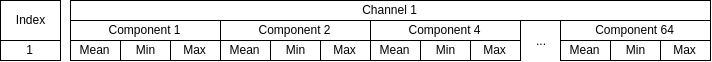
\includegraphics[width=\linewidth]{images/structure}
	\caption{The structure of each row of the CSV file which is repeated for minimum and maximum values.}
	\label{fig:structure}
\end{figure}

The mean, min, and max values were plotted for each channel for each sensor. The plots of the means of each channel for the book and plastic case objects are shown in figures \ref{fig:book} and \ref{fig:plasticcase} respectively. The difference between the resulting signals from the two objects are very clear.

\begin{figure}[!ht]
	\centering
	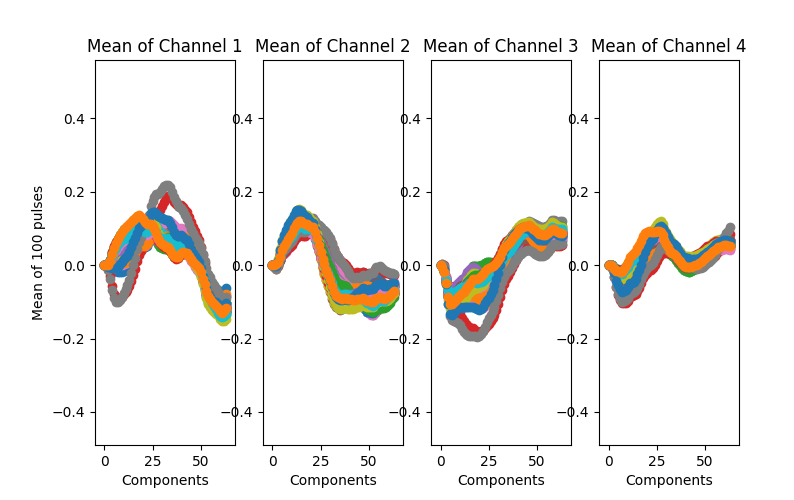
\includegraphics[width=\linewidth]{images/book}
	\caption{Mean of each channel measured for the book}
	\label{fig:book}
\end{figure}

\begin{figure}[!ht]
	\centering
	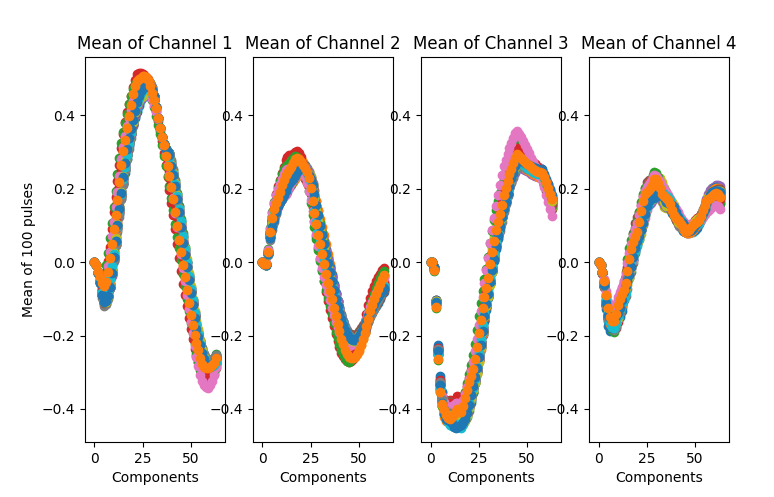
\includegraphics[width=\linewidth]{images/plasticcase}
	\caption{Mean of each channel measured for the plastic case}
	\label{fig:plasticcase}
\end{figure}

In the binary dataset, the minimum and maximum components observed all followed a similiar shape as the average, but the book class did contain one severe outlier in two plots. The full plots are included in the submission under \url{plots/binarybook.png} and \url{plots/binaryplasticcase}, in which the plot of the minimum components in channel one and the maximum components in channel three both include one row of outliers. 
Since the average did not deviate from other components for that class, it seemed fair to say that these maximum and minimum readings were outliers. Instead of removing them and risking producing a biased model, the row was left in the data set. A real world application of the sensor would likely involve noise, and so it made sense to train the model to be able to cope with anomalies. The existence of these outliers was however noted when choosing a cost function however in order to try and minimise their affect.

The same plots were made for the multiclass dataset, and from this it was clear that each material produced very different results, with varying levels of consistency. For example, the data aquired when the radar sensor was applied to a human hand varied wildly, whilst the readings for the plastic cover were a very clear sinusoidal shape. These plots can be found in \url{plots/multiclass*}.

Since the radar signature was determined by the reflection of the radar pulses on the surface and interior structure of each object, the resulting plots were understandable. For example, the plastic case shows a very consistent pattern likely due to the fact that it is composed of a single material in a uniform structure, whilst the human hand produces a very chaotic signature since it is composed of many different materials, especially fluids in motion.

\begin{figure}
\centering
\begin{subfigure}{.5\textwidth}
  \centering
  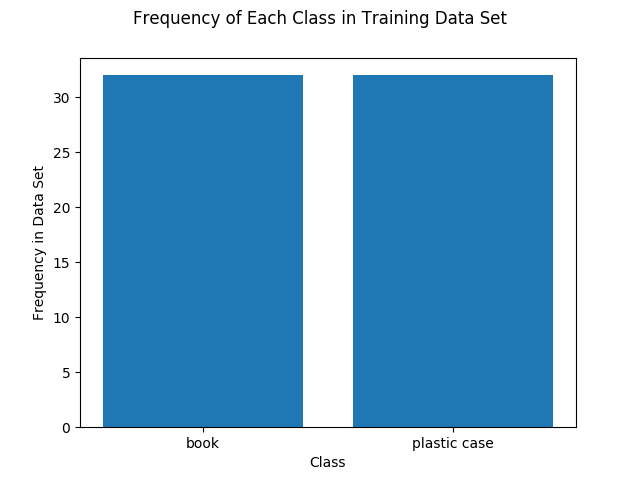
\includegraphics[width=\linewidth]{images/binaryfrequencies}
  \caption{Binary}
  \label{fig:sub1}
\end{subfigure}%
\begin{subfigure}{.5\textwidth}
  \centering
  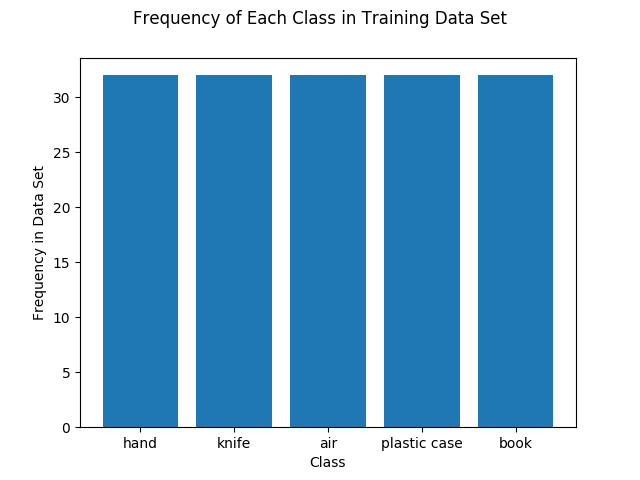
\includegraphics[width=\linewidth]{images/multiclassfrequencies}
  \caption{Multiclass}
  \label{fig:sub2}
\end{subfigure}
\caption{Frequencies of each class in the binary and multiclass training data sets}
\label{fig:classdist}
\end{figure}

The training data set was shown not be skewed by plotting the distribution of each class (figure\ref{fig:classdist}). The equal distribution of each class meant that cross validation of a classifier that always guesses the same class will have a ratio of correct predictions inversely proportional to number of classes in the training data set. 

All data from the feature set had values between -1 and 1, and from the plots of all classes it was noticed that the different classes had different global minumum and maximums for each channel. For example, the components of samples for air did not surpass 0.1, 0.25 for books, 0.5 for plastic case, and 0.75 to 1 for hand and knife. Based on this normalisation was used over standardisation, as there were no outliers and the values were fairly evenly distributed. Plotting the normalised data and comparing it to the plots of the original data reinforced this decision, as the shape and scale of the resulting plots had bbeen maintained.

\section{Feature Selection}

The large number of features available in the dataset makes computation of any model especially expensive. In order to have an effective classifier, there should be at least five examples of each combination of values in the training data \cite{mincombs}, which our dataset is unable to provide. Therefore a reduction of the feature set was considered.

The visualisations of the training data showed that each class had very different levels of variation between each sample, and this variation could be used to identify a class. Since our model would need to identify the class based on a single sample, this variation could not be relied on. 

\section{Model Selection and Training}

Multiclass classifcation can be implemented using binary classifiers by training an individual classifier for each class, and each classifier is only able to state if the input represents its class or not. Since the training data used has an equal distribution of each class, each classifier would be trained on skewed data with far more negatives than positives as demonstrated in figure \ref{fig:classifierperclass}. This method would require as many classifiers as there are classes, and is referred to as the one-vs-all method \cite{handson}.

\begin{figure}[!ht]
	\centering
	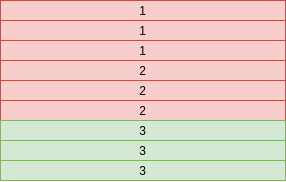
\includegraphics[width=0.5\linewidth]{images/classifierperclass}
	\caption{Distribution of negative and positive samples for a classifier trained to identify either class '3' or 'not 3' when each class is equally represented}
	\label{fig:classifierperclass}
\end{figure}

Another method is called the one-vs-one classifier, where a classifier exists for each pair of classes. Each classifier will predict a value from the two classes it was trained to identify, and the resulting prediction will be the class that was chosen by the most classifiers. This method requires $n (n - 1)^2$ classifiers, where n is the number of classes.

There also exist dedicated multiclass classifiers with different advantages and implementations.

Since the RadarCat \cite{radarcat} technology is intended to be able to allow users to identify and catalogue various every day objects, both the one-vs-one and one-vs-all approaches would involve a large number of classifiers being trained. Therefore an approach that required fewer classifiers would probably be preferred. 

On the other hand, the Soli \cite{soli} technology used by RadarCat was designed with the intention of recognising hand gestures, and would so being able to generalise well with fewer classes would likely be favoured in that case (i.e. handling many variations of the same hand gesture).

Another possible solution that could reduce the number of classifiers needed as the number of classes grow is to create a hierarchy of classifiers. Each node has an "is-a" relationship with its parent in the tree, and prediction involves starting with a very generic classifier, and gradually getting more specific. \cite{heirarchy} for example used such classifier to identify the musical genre of an audio clip using a heirachical structure. Though it performed similiarly to a flat classifier approach, it would be easier to include new classes. This would be useful for the RadarCat use case as the number of objects it is used to identify grows.

The ability to provide online learning (or at least batch learning) would also be useful, as user feedback could provide a method for crowdsourcing samples for further supervised learning. Crowdsourced data collection for producing data for supervised learning has famously been applied by projects such as reCAPTCHA \cite{captcha}, and a similiar method could be used by RadarCat to improve its error rate.

With the previous information in mind (and for the sake of evaluation and comparison), an inherently multiclass method (Random Forest) and a one-vs-all method (Linear Support Vector Classification) were chosen for the first and second models respectively. 

\subsection{Model 1: Random Forest Classifier}

The random forest classifier was chosen due to its robustness when dealing with noisy data, which would definitely be present in real world applications \cite{rf}. The number of classifiers would remain static as the number of classes grow, though training would be slower, especially due to the high number of dimensions.



\subsection{Model 2: Linear Support Vector Classifier}

The one-vs-all LSVC was chosen as it scales well as the number of samples increases.

\section{Evaluation and Comparison}
\section{Discussion}

\bibliographystyle{unsrt}
\bibliography{mybib}

\end{document}
